%!TEX root=../document.tex

\section{Verbaute Grafikkarten}


\subsection{Geräte-Manager}
Im Geräte-Manager sind die verbauten Grafikkarten vorzufinden

\begin{minipage}{\linewidth}
	\centering
	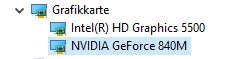
\includegraphics[width=0.8\linewidth]{images/graka}
	\figcaption{Verbaute Grafikkarten im Geräte-Manager}
\end{minipage}

\subsection{Datenblatt}
Es ist auch im Datenblatt, für meinen Laptop, nachzulesen welche Grafikkarten verfügbar sind:


\begin{minipage}{\linewidth}
	\centering
	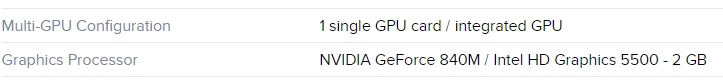
\includegraphics[width=0.8\linewidth]{images/graka2}
	\figcaption{Verbaute Grafikkarten im Laptop-Datenblatt}
\end{minipage}

\subsection{Fazit}
Es ist eine Tatsächliche Grafik\textbf{karte} verbaut und eine integrierte Graphics Processing \textbf{Unit}, und zwar:

\begin{itemize}
	\item \verb|NVIDIA GeForce 840M|
	\item \verb|Intel(R) HD Graphics 5500|
\end{itemize}

\clearpage
\section{NVIDIA GeForce 840M}
Es sind folgende Spezifikationen auf der offiziellen \underline{\href{https://www.geforce.com/hardware/notebook-gpus/geforce-840m/specifications}{Nvidia Website}} vorhanden:

\begin{minipage}{\linewidth}
	\centering
	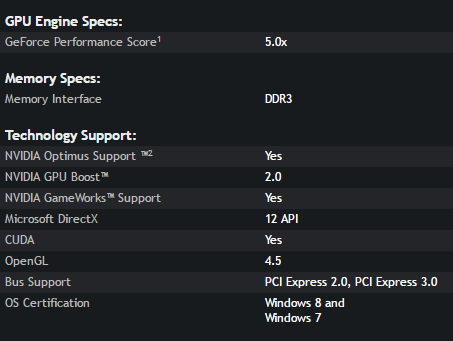
\includegraphics[width=0.8\linewidth]{images/nvidia_specs}
	\figcaption{Datenblatt der Grafikkarte auf der Nvidia seite}
\end{minipage}

Dieses Datenblatt gibt allerdings nicht genügend Info, besonders was den Speicher angeht. Von einer \underline{\href{http://laptopmedia.com/video-card/nvidia-geforce-840m-2gb-ddr3/}{Testing-Website (laptopmedia.com)}} konnten noch folgende Informationen herausgelesen werden:

\begin{minipage}{\linewidth}
	\centering
	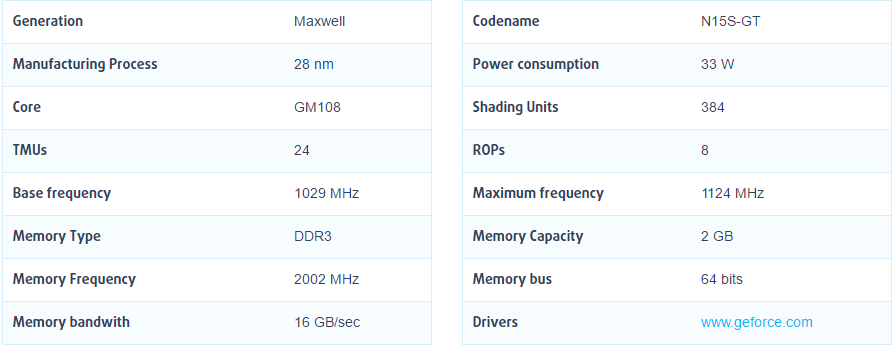
\includegraphics[width=0.8\linewidth]{images/specs}
	\figcaption{Datenblatt der Grafikkarte auf einer Testing-Website}
\end{minipage}

\section{Intel(R) HD Graphics 5500}
Für die integrierte Grafikeinheit konnten folgende Informationen von \underline{\href{https://www.notebookcheck.net/Intel-HD-Graphics-5500.125586.0.html}{notebookcheck.net}} herausgefunden werden:
	
\begin{minipage}{\linewidth}
	\centering
	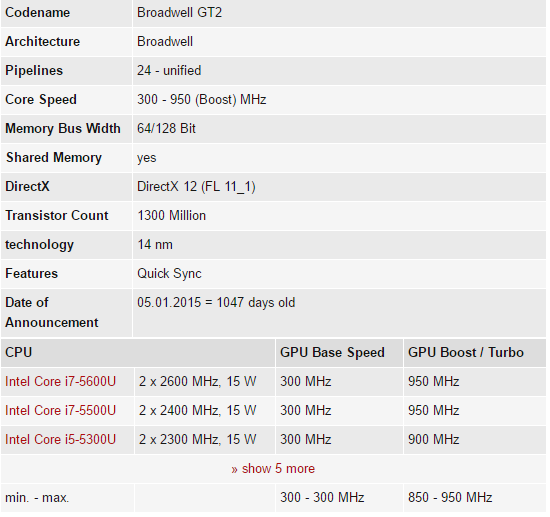
\includegraphics[width=0.8\linewidth]{images/gpu_specs}
	\figcaption{Datenblatt der integrierten Grafikeinheit}
\end{minipage}

\section{Entwicklungsumgebung}
Da auf der Grafikkarte gearbeitet wird, welche von \verb|Nvidia| hergestellt ist, wird mit \verb|CUDA| gearbeitet. \verb|CUDA| wird direkt von \verb|Nvidia| unterstützt und bietet auch eine große Community und Support.

